\documentclass[accentcolor=tud9c]{tudexercise}

\usepackage{amsmath}
\usepackage{graphicx}
\usepackage{listings}


\title{Machine learning\\Homework 1}
\author{David Gr\"omling 1806724}
%\maketitle

\newcommand{\mat}[3]{
	\begin{pmatrix}
	#1_{11} & \cdots & #1_{1#3} \\
	\vdots	& \ddots & \vdots \\
	#1_{#21}	& \cdots & #1_{#2#3}
	\end{pmatrix}
}

\newcommand{\matplus}[4]{
	\begin{pmatrix}
		#1_{11} + #2_{11} & \cdots & #1_{1#4} + #2_{1#4}\\
		\vdots	& \ddots & \vdots \\
		#1_{#21} + #2_{#21}	& \cdots & #1_{#3#4} + #2_{#3#4}
	\end{pmatrix}
}

\newcommand{\matmult}[5]{
		\begin{pmatrix}
			\sum_{k=1}^{#4} #1_{1k} \cdot #2_{k1} & \cdots & \sum_{k=1}^{#4} #1_{1k} \cdot #2_{k#5}\\
			\vdots	& \ddots & \vdots \\
			\sum_{k=1}^{#4} #1_{#3k} \cdot #2_{k1}	& \cdots & \sum_{k=1}^{#4} #1_{#3k} \cdot #2_{k#5}
		\end{pmatrix}
	}


\begin{document}
	
	
	\section{Linear Algebra Refresher}
	Rene Wilmes (2862149), David Gr\"omling (1806724)
	\subsection{Matrix Properties}
	
	Not all properties of scalars are valid for matrices. To proove this, the following definitions are used:
	
	$ A = \mat{a}{m}{n} $, $ B = \mat{b}{m}{n} $, $ C = \mat{c}{n}{l} $


	\subsubsection{Commutative}
	\textbf{Addition}
	
	Show $ A+B \stackrel{!}{=} B+A$
	
	Using the commutative law of scalar addition yields:
	\[ A + B = \matplus{a}{b}{m}{n} \stackrel{scalar}{=} \matplus{b}{a}{m}{n} = B + A \]
	
	Matrix addition is commutative\\
	
	\noindent \textbf{Multiplication}
	Show $ A*C \stackrel{!}{=} C*A$
	
	$ A_{m x n} * C_{i x j} $ only defined for matrices that fulfill $ n = i $. Therefore, $  C_{i x j} * A_{m x n} $ only possible for $ j = m $.
	
	Even in that case, $A*C = C*A$ is not generally true, as the following equation shows.
	\[ A*C = \matmult{a}{c}{m}{n}{m} \stackrel{generally}{\neq}  \matmult{c}{a}{m}{n}{m} = C * A \]
	
	Matrix multipllication is NOT commutative.
	
	\subsubsection{Distributive}
	Show $ (A + B) * C \stackrel{!}{=} A*C + B*C $
	
	Using the scalar version of the distributive law yields:
	
	$ (A+B)*C\\= \matplus{a}{b}{m}{n} * \mat{c}{n}{l}\\ = \matmult{(a+b)}{c}{m}{n}{l}\newline
	 \stackrel{scalar}{=} \matmult{a}{c}{m}{n}{l} + \matmult{b}{c}{m}{n}{l}\\
	 = A*C + B*C $
	 
	 Matrix operations are distributive.
	 
	 \subsubsection{Associative}
	 \textbf{Addition} (In this section, $A,B,C \in \Re^{m x n}$ )
	 
	 Show $A + (B + C) = (A+B) + C $
	 
	 Using the scalar version of the associative law yields:
	 
	 $A + (B + C)\\
	 = A + \matplus{b}{c}{m}{n}\\
	 = \matplus{a}{(b+c)}{m}{n}\\
	 \stackrel{scalar}{=} \matplus{(a+b)}{c}{m}{n}\\
	 = \matplus{a}{b}{m}{n} + C
	 = (A+B) + C$
	 
	 Matrix addition is associative.
	 
	 \noindent \textbf{Multiplication} (In this section: $A \in \Re^{mxn}, B \in \Re^{nxi}, C \in \Re{ixj}$)
	 
	 Show $ A*(B*C) = (A*B)*C $
	 
	 At element (i,l) of the product:\\

	 $ \sum_{j=1}^{n} a_{ij} (\sum_{k=1}^{m} b_{jk}\cdot c_{kl})\\
	 = \sum_{j=1}^{n}\sum_{k=1}^{m} a_{ij}b_{jk}c_{kl}\\
	 \stackrel{commutative}{=} \sum_{k=1}^{m} \sum_{j=1}^{n} a_{ij}b_{jk}c_{kl}\\
	 = \sum_{k=1}^{m} c_{kl} (\sum_{j=1}^{n} a_{ij} \cdot b_{jk} )
	 $
	 
	 Matrix multiplication is associative.
	 
	 \subsection{Matrix Inversion}
	 
	 $ A = \begin{pmatrix} 
			 1 & 2 & 3 \\
			 1 & 2 & 4 \\
			 1 & 4 & 5 \\
		   \end{pmatrix}
	 $
	 
	 \noindent \textbf{Inversion} (Gauss)\\
	 $
	 \begin{pmatrix} 
	 1 & 2 & 3 & \vline & 1 & 0 & 0\\
	 1 & 2 & 4 & \vline & 0 & 1 & 0\\
	 1 & 4 & 5 & \vline & 0 & 0 & 1\\
	 \end{pmatrix}
	 \stackrel{(2) = (2)-(1), (3) = (3)-(1)}{->}\\
	 \begin{pmatrix} 
	 	 1 & 2 & 3 & \vline & 1 & 0 & 0\\
	 	 0 & 0 & 1 & \vline & -1 & 1 & 0\\
	 	 0 & 2 & 2 & \vline & -1 & 0 & 1\\
	 \end{pmatrix}
	 \stackrel{(1) = (1)-(3), (3)=[(3)-2(2)]/2}{->}\\
	 \begin{pmatrix} 
	 	 1 & 0 & 1 & \vline & 2 & 0 & -1\\
	 	 0 & 0 & 1 & \vline & -1 & 1 & 0\\
	 	 0 & 1 & 0 & \vline & 0.5 & -1 & 0.5\\
	 \end{pmatrix}
	 \stackrel{(1)=(1)-(2), (2)=(2)-(3)}{->}\\
	 \begin{pmatrix} 
		1 & 0 & 0 & \vline & 3 & -1 & -1\\
		0 & -1 & 1 & \vline & -1.5 & 2 & -0.5\\
		0 & 1 & 0 & \vline & 0.5 & -1 & 0.5\\
	 \end{pmatrix}
	 \stackrel{(3)=(2)+(3)}{->}\\
	 \begin{pmatrix} 
		 1 & 0 & 0 & \vline & 3 & -1 & -1\\
		 0 & -1 & 1 & \vline & -1.5 & 2 & -0.5\\
		 0 & 0 & 1 & \vline & -1 & 1 & 0\\
	 \end{pmatrix}
	 \stackrel{(2)=-[(2)-(3)]}{->}\\
	 \begin{pmatrix} 
	 1 & 0 & 0 & \vline & 3 & -1 & -1\\
	 0 & 1 & 0 & \vline & 0.5 & -1 & 0.5\\
	 0 & 0 & 1 & \vline & -1 & 1 & 0\\
	 \end{pmatrix}	 
	 $
	 
	 $A^{-1} = \begin{pmatrix} 
	 3 & -1 & -1\\
	 0.5 & -1 & 0.5\\
	 -1 & 1 & 0\\
	 \end{pmatrix} $
	 \\\\
	 
	 
	  $ A = \begin{pmatrix} 
	  1 & 2 & 3 \\
	  1 & 2 & 4 \\
	  1 & 2 & 5 \\
	  \end{pmatrix} $ is not invertible because columns 1 and 2 are linearly dependent. In less obvious cases one could also check if the determinant $det(A)$ equals 0. In that case $A$ is not invertable:	  
	\begin{align*}
	det(A) &= 1*2*4 + 1*2*5 + 1*2*3 - 1*2*4 - 1*2*3 -1*2*5 \\
	&= 8 + 10 + 6 - 8 - 6 - 10 \\
	&= 0
	\end{align*}\\
	
	\subsection{Matrix Pseudoinverse}
	Definition of right and left pseudoinverse of a generic matrix $A$ with dimension $n\, \times \, m$:\\
	\[A^{-1}_{left} = (A^{T}A)^{-1}A^{T}, so\; that\; A^{-1}_{left}A=I_{m}\\ \]
	\[A^{-1}_{right} = A^{T}(AA^{T})^{-1}, so\; that\; A^{-1}_{right}A=I_{n}\]
	Note that $I_k$ denotes the $k\, \times \, k$ identity matrix.\\
	\\
	In order to determine $A^{-1}_{left}$ and $A^{-1}_{right}$ of a matrix $A \in \Re^{2\times 3}$ we can compute the following matrices in the intermediate steps:\\
	For $A^{-1}_{left}$:	
	\begin{align*}
	A^{T} &\in \Re^{3 \times 2} \\
	A^{T}A &\in \Re^{3 \times 3} \\
	(A^{T}A)^{-1} &\in \Re^{3 \times 3} \\
	(A^{T}A)^{-1}A^{T} &\in \Re^{3 \times 2}
	\end{align*}
	For $A^{-1}_{right}$:	
	\begin{align*}
	A^{T} \in \Re^{3 \times 2} \\
	AA^{T} \in \Re^{2 \times 2} \\
	(AA^{T})^{-1} \in \Re^{2 \times 2} \\
	A^{T}(AA^{T})^{-1} \in \Re^{3 \times 2}
	\end{align*}
	
	\subsection{Eigenvectors and Eigenvalues}
	Eigenvectors $v_n$ of a Matrix $M$ fullfill $\alpha_n  v_n = Mv_n $ with $\alpha_n \in \Re$. $\alpha_n$ is called Eigenvalue of $M$. In machine learning one has to cope with a lot of data, which can be seen as a high-dimensional vector space. Dealing with high dimensions can be very ressource intensive. Eigenvalues and eigenvectors indicate which dimensions have a high variance and therefore offer the \emph{most} information about the data, allowing one to rank the dimensions and possibly reduce the vector space by filtering less useful dimensions.
	
	\section{Statistics Refresher}
	\subsection{Expectation and Variance}
	\textbf{1)}
	$ E(\Omega) = \sum_{\omega \in \Omega} p(\omega)\omega$
	
	$Var(\Omega) = {\sum_{\omega \in \Omega} p(\omega)(\omega - E(\Omega))^2}$
	
	The expectation is linear, $ E(X+Y) = E(X) + E(Y) $. Because of the quadratic term in the variance, the variance is non-linear.
	
	\noindent \textbf{2)}\\
	Dice A:\\
	
	$ E(A) \approx \frac{1}{6} (3 \cdot 4 + 2 \cdot 1 + 1 \cdot 2)  = \frac{1}{6} \cdot 16 = \frac{8}{3} \approx 2.67$\\
	
	$ Var(A) \approx \frac{1}{6-1} [3 \cdot (4-\frac{8}{3})^2 + 2 \cdot (1-\frac{8}{3})^2 + 1 \cdot (2-\frac{8}{3})]\\
	= \frac{1}{5} [3\cdot (\frac{4}{3}) ^2 + 2\cdot (\frac{5}{3}) ^2 + (\frac{2}{3}) ^2]\\
	= \frac{1}{5}[\frac{48+50+4}{9}] = \frac{102}{45} = \frac{34}{15} \approx 2.27$\\
	
	\noindent Dice B:\\
	
	$E(B) \approx \frac{1}{6}(4 \cdot 3 + 4 +6) = \frac{1}{6} \cdot 22 = \frac{11}{3} \approx 3.67 $\\
	
	$ Var(B) = \frac{1}{5}(4\cdot (3-\frac{11}{3})^2 + (4-\frac{11}{3})^2 + (6-\frac{11}{3})^2 )\\
	= \frac{16+1+49}{45} = \frac{22}{5} = 4.4 $\\
	
	\noindent Dice C:\\
	
	$E(C) \approx \frac{1}{6} \cdot (2 \cdot 5 + 2 + 3 \cdot 1) = \frac{15}{6} = \frac{5}{3} \approx 1.67 $\\
	
	$Var(C) \approx \frac{1}{5} \cdot (2 \cdot (5-\frac{5}{3})^2 + (2-\frac{5}{3})^2 + 3 \cdot (1- \frac{5}{3})^2) \\
	= \frac{1}{5} \cdot \frac{200+1+12}{9} = \frac{71}{15} \approx 4.73$
	
	\noindent \textbf{3)}\\
	The most rigged dice is dice C, since its mean differs most from the expected $\frac{1}{6} \cdot \sum_{i=1}^6 i = 3.5 $
	
	\subsection{It's a cold world}
	a)\\
	has cold: C\\
	has backpain: B\\
	\\
	b)\\
	Both random variables are binary: True and false\\
	\\
	c)\\
	$ P(B|C) = 30 \% $\\
	$ P(C) = 5 \% $ \\
	$ P(B|\bar{C})  = 10\%$\\
	\\
	d)\\
	Looking for $P(C|B) = \frac{P(C,B)}{P(B)}$ \\
	$ P(B,C) = P(B|C) \cdot P(C) = 30\% \cdot 5\% = 1.5\% $ \\
	$ P(\bar{C}) = 1-P(C) = 0.95 $\\
	$ P(B, \bar{C}) = P(B|\bar{C}) \cdot P(\bar{C}) = 10 \% \cdot 95\% = 9.5 \%$\\
	$ P(B) = P(B,C) + P(B,\bar{C}) = 1.5\% + 9.5\% = 11\% $
	$ P(C|B)= \frac{P(C,B)}{P(B)} = \frac{1.5\%}{11\%} = 13.6\% $ 
	
	The chance that some with a backpain has a cold is 13.6 \%.
	
	\subsection{Deadly Virus}
	$ s_{t+1} = \begin{pmatrix}
	 0.35 & 0.015\\
	 1-0.35 & 1-0.015
	\end{pmatrix} \cdot s_t = \begin{pmatrix}
	0.35 & 0.015\\
	0.65 & 0.985
	\end{pmatrix} \cdot s_t $
	
	
	\section{Optimization and Information Theory}
	\subsection{Entropy}
	Definition of Entropy: $ H = -\sum_{n} p_n log_2(p_n)$
	
	With sample data: $ H = -0.01 \cdot log_2(0.01) - 0.65 \cdot log_2(0.65 - 0.25 \cdot log_2(0.25)) - 0.09 \cdot log_2(0.09) bit\\
	 = 1.2831 bit
	$
	
	Since only full integer numbers of bits can be transmitted, the minimum number of required bits to transmit one symbol is ceil(1.2831)bit = 2bit
	
	
	\subsection{Constrained Optimization}
	\begin{enumerate}
	\item %additional constraint & formulation
	In order to gain a useful solution we have to add one additional constrained, which makes sure that however we choose the probabilities we maintain a valid probability distribution. That means all probabilities have to sum up to 1:
	\[	\sum_{i=1}^4p_{i}=1\]
	Formulating it as a constrained optimization problem requires us to transform the constraints and set them to zero. Let $f$ be the function we want to maximize and $g_1$, $g_2$ our constraints as follows:
	\begin{align*}
	f(p_1,p_2,p_3,p_4) &=-\sum_{i=1}^4p_ilog_2(p_i) \\
	&=-(p_1log_2(p_1)+p_2log_2(p_2)+p_3log_2(p_3)+p_4log_2(p_4)) \\
	g_1(p_1,p_2,p_3,p_4) &=-4+\sum_{i=1}^42p_ii \\
	&= p_1 + 2p_2 + 3p_3 + 4p_4 - 2 \\
	g_2(p_1,p_2,p_3,p_4) &=-1+\sum_{i=1}^4p_i \\
	&= p_1 + p_2 + p_3 + p_4 - 1
	\end{align*}
	We then get our constrained optimization problem:
	\begin{align*}
	f(p_1,p_2,p_3,p_4) & \rightarrow MAX\\
	g_1(p_1,p_2,p_3,p_4) & = 0 \\
	g_2(p_1,p_2,p_3,p_4) & = 0
	\end{align*}
	\item %lagrangian
	We get our lagrangian from the general form:
	\[
		L(x_1,...,x_n,\lambda_1,...,\lambda_k) = f(x_1,...,x_n) + \lambda_1 \cdot g_1(x_1,...,x_n) +\, \cdot \cdot \cdot \, + \lambda_k \cdot g_k(x_1,...,x_n)
	\]
	Therefore:
	\begin{align*}
		L(p_1,p_2,p_3,p_4,\lambda_1, \lambda_2) &= f(p_1,p_2,p_3,p_4) + \lambda_1 \cdot g_1(p_1,p_2,p_3,p_4) + \lambda_2 \cdot g_2(p_1,p_2,p_3,p_4) \\
		&= -p_1log(p_1) -p_2log(p_2) -p_3log(p_3) -p_4log(p_4) \\
		&\quad \quad + \lambda_1p_1 + 2\lambda_1p_2 + 3\lambda_1p_3 + 4\lambda_1p_4 - 2\lambda_1 \\
		&\quad \quad + \lambda_2p_1 + \lambda_2p_2 + \lambda_2p_3 + \lambda_2p_4 - \lambda_2
	\end{align*}
	
	\item %derivatives
	We have to compute 6 partial derivatives, one for each variable $p_1,...,p_4$ and one for each lagrangian multiplier $\lambda_1$ and $\lambda_2$. The derivatives look as follows:
	\begin{align*}
	\frac{\delta L}{\delta p_1} &= -log_2(p_1) - \frac{1}{ln(2)} + \lambda_1 + \lambda_2 \\
	\frac{\delta L}{\delta p_2} &= -log_2(p_2) - \frac{1}{ln(2)} + 2\lambda_1 + \lambda_2 \\
	\frac{\delta L}{\delta p_3} &= -log_2(p_3) - \frac{1}{ln(2)} + 3\lambda_1 + \lambda_2 \\
	\frac{\delta L}{\delta p_4} &= -log_2(p_4) - \frac{1}{ln(2)} + 4\lambda_1 + \lambda_2 \\
	\frac{\delta L}{\delta \lambda_1} &= p_1 + 2p_2 + 3p_3 + 4p_4 - 2 \\
	\frac{\delta L}{\delta \lambda_2} &= p_1 + p_2 + p_3 + p_4 - 1
	\end{align*}
	This leads us to the following linear system of equations:
	\begin{align}
	0 &= -log_2(p_1) - \frac{1}{ln(2)} + \lambda_1 + \lambda_2 \\
	0 &= -log_2(p_2) - \frac{1}{ln(2)} + 2\lambda_1 + \lambda_2 \\
	0 &= -log_2(p_3) - \frac{1}{ln(2)} + 3\lambda_1 + \lambda_2 \\
	0 &= -log_2(p_4) - \frac{1}{ln(2)} + 4\lambda_1 + \lambda_2 \\
	0 &= p_1 + 2p_2 + 3p_3 + 4p_4 - 2 \\
	0 &= p_1 + p_2 + p_3 + p_4 - 1
	\end{align}
	The usual approach would be to transform the first four equations (1) - (4) to get values for $p_i$ and insert them in (5) and (6) to eventually get values for $\lambda_1$ and $\lambda_2$. However an analytical solution is hard to obtain because transforming (1) - (4) will lead to exponential functions which can not be eliminated. Therefore it is a non-linear equation system.
	\item %dual function
	Given a our lagrangian function $L$ from above the lagrange dual function is defined as follows:
	\[
		\theta (v, \lambda) = \inf_{x\in D} L(x, v, \lambda) = \inf_{x\in D}\left( f_0(x) + \sum_{i=1}^{p}v_if_i(x) + \sum_{i=1}^{m}\lambda_i g_i(x)\right)
	\]
	Where $D$ denotes the domain which the values of $x$ are taken from, and $v_i$ are lagrangian multipliers from inequality constraints (which are not present in our case). We deduce the following dual function $\theta^{*}$ for our case:
	\begin{align*}	
		\theta^{*} (\lambda) &= \inf_{x\in D} L(x, \lambda) \\
		&= \inf_{x\in D} \left( f_0(x) + \sum_{i=1}^{m} \lambda_i g_i(x) \right) \\
		&=  \inf_{x \in D} \left( f(x) + \lambda_1 \cdot g_1(x) + \lambda_2 \cdot g_2(x) \right) \\
		&=  \inf_{p_1,p_2,p_3,p_4 \in D} \left( f(p_1,p_2,p_3,p_4) + \lambda_1 \cdot g_1(p_1,p_2,p_3,p_4) + \lambda_2 \cdot g_2(p_1,p_2,p_3,p_4) \right) \\
		&= \inf_{p_1,p_2,p_3,p_4 \in D} (-p_1log(p_1) -p_2log(p_2) -p_3log(p_3) -p_4log(p_4) \\
		&\quad \quad \quad \quad \quad \quad \quad + \lambda_1p_1 + 2\lambda_1p_2 + 3\lambda_1p_3 + 4\lambda_1p_4 - 2\lambda_1 \\
		&\quad \quad \quad \quad \quad \quad \quad + \lambda_2p_1 + \lambda_2p_2 + \lambda_2p_3 + \lambda_2p_4 - \lambda_2)
	\end{align*}
	The dual function $\theta$ is a concave function by its composition from affine functions. Therefore it can also be viewed as a convex function (if $\theta$ is concave then $-\theta$ is convex) and leads to a convex optimization problem. In general there are no analytical solutions to this problem, however one may apply certain numerical techniques.
	\item %numerical solution
	In order to numerically solve this problem one could use the steepest descent algorithm. That algorithm starts at an (arbitrary or specifically chosen) initial point and computes the gradient (which is a vector pointing towards the maximum ascend). Then one moves to another point in the opposite direction direction of the gradient with a given (or computed) stepsize. This is done repeatedly until one reaches a local minimum (or is satisfactory close to it).

	\end{enumerate}
	
	\subsection{Numerical Optimization}
	The learning rate has a huge impact on the algorithms performance. We made different tests with a constant and dynamic learning rates, see figure \ref{fig:GDA-curve}. While the best performing constant rate $a_0$ learns way faster in the first 60-70 iterations, the dynamic rate $a_1$ catches up and ultimately converges faster towards 0. Figures \ref{code:python1} and \ref{code:python2} show our used python code.
	\begin{figure} [h]
	\centering
	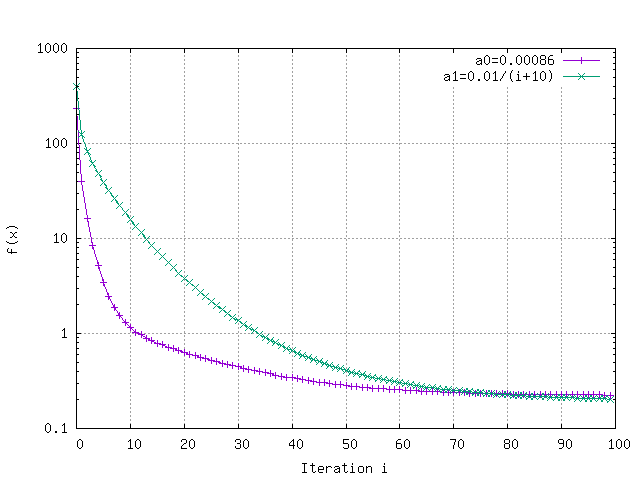
\includegraphics [scale=0.65] {value_logscale.png}
	\caption{Learning curves from initial point $(2,2,...,2)$.}
	\label{fig:GDA-curve}
	\end{figure}
	
	\begin{figure} [h]
	\begin{lstlisting}
#!/usr/local/bin/python2.7

import sys
import numpy as np

# main function
def main(argv):
	# params
	steps = argv[0]
	learnRate = float(argv[1])
	
	n = 20

	# init data array
	x = []
	for i in range(0, int(n)):
		x.append(2)

	for i in range(0, int(steps)):
		# adjust learning rate here
		#rate = learnRate/(i+10)
		rate = learnRate

		# compute gradient
		grad = getGradient(x)

		# update x
		x = updateX(x, rate, grad)
		
		# print f(x)
		print(str(i) + "\t" + str(f(x)))

	# exit
	sys.exit()

# updates the date given the learn-rate and gradient 
def updateX(x, learnRate, grad):
	for j in range(0, len(x)):
		x[j] = x[j] - learnRate * grad[j]

	return x
	\end{lstlisting}
	\caption{Gradient descent python code snippet 1 of 2.}
	\label{code:python1}
	\end{figure}
	
	
	\begin{figure} [h]
	\begin{lstlisting}
# computes the rosenbrocks function
def f(x):
	sum = 0
	for i in range(0, len(x)-1):
		sum += 100*np.power((x[i+1]-x[i]*x[i]), 2)
		sum += np.power((x[i] - 1), 2)
	return sum

# computes the gradient
def getGradient(x):
	length = len(x)
	list = []
	for i in range(0, length):
		list.append(getFirstDerivative(x, i))
	
	# return list
	grad = np.array(list)
	grad = np.transpose(grad)
	return grad
	
# returns the first derivative of the rosenbrocks function
def getFirstDerivative(x, i):
	length = len(x)
	
	if (i == 0):
		# i==0
		x0 = x[i]
		return -400*x0*(x[i+1]-x0*x0)+2*(x0-1)
	elif (i == length-1):
		# i==N
		return 200*(x[i]-np.power(x[i-1], 2))
	else:
		# 0 < i < N
		x0 = x[i]
		y = x[i+1]
		z = x[i-1]

		return -400*x0*(y-x0*x0)+200*(x0-z*z)+2*(x0-1)

if __name__ == "__main__":
	main(sys.argv[1:])	
	\end{lstlisting}
	\caption{Gradient descent python code snippet 2 of 2.}
	\label{code:python2}
	\end{figure}
	
	\subsection{Gradient Descent Variants}
	There are three main variants of gradient descent.
	\begin{itemize}
		\item 	Batch gradient descent: This is the simplest version of gradient descent. At each iteration, it computes the gradient of the loss function globally. This comes at the cost of very high memory usage, since the whole dataset needs to be kept in memory at every iteration. Therefore, this algorithm is hardly used without the following two optimizations
		\item Stochastic gradient descent (SGD): The first step of SGD is to shuffle the dataset. Then, instead of computing the global gradient of the loss function, SGD calculates the loss function with respect to the current sample and then moves on to the next sample until all samples were passed. This process is repeated until the end-criteria is met. The advantage of this approach is that it requires less computation resources than batch gradient descent, since only one sample has to be kept in memory. However, the optimization for one sample can lead to jumps in the global loss function, which is often not desired.
		\item Mini-batch gradient descent: This optimization takes the best of both worlds. The main difference to SDG is, that is minimizes the loss-function for a number of samples at a time and therefore prevents big errors introduced by some samples. However, since the number of chosen samples is typically small, compared to the whole sample set, it is still computationally efficient.
	\end{itemize}

	Momentums are a fraction of the last update vector that are added to the current update vector. This is especially useful in areas with a steep curvature in one dimension and a low one in the other. In such a situation, momentum prevents oscillation and accelerates convergence. However, in situations of a broad "valley" with steep turns towards the minimum, the momentum has a negative effect.
		
\end{document}